\documentclass[11pt,a4paper]{report}
\usepackage[utf8]{inputenc}
\usepackage[english]{babel}
\usepackage{amsmath}
\usepackage{enumitem}
\usepackage{amsfonts}
\usepackage{pdfpages}
\usepackage{titlesec}
\titlespacing*{\chapter}{0pt}{0pt}{30pt}
%\usepackage[Glenn]{fncychap}
\usepackage{amssymb}
\usepackage[left=2.5cm,right=2.5cm,top=2cm,bottom=2.5cm]{geometry}
\title{Architectural Design }
\author{
Matthias Tavasszy \\
\texttt{4368401}	
\and
Arjan van Schendel \\
\texttt{4366212}
\and
Luke Prananta \\ 
\texttt{4288386}  
\and
Jasper van Esveld \\
\texttt{4372581}
\and
Bart Ziengs \\ 
\texttt{4391799}
}

\begin{document}

\maketitle


\tableofcontents
\chapter*{Introduction}
\section*{Design Goals}
The design goals are things we want to accomplish in terms of our design of the product.
These can be divided in several categories.
\subsection*{Fully tested and integrated}
Every week a working build is produced with high coverage testing and integration with
Unity Cloud Build. We must ensure that a user will not experience any system breakdowns or
bugs. The people who will use our system are often mentally fragile and any negative
experience can have long­lasting or permanent negative consequences.
\subsection*{Performance}
Immersion is a key part of virtual reality and to get the best experience we need to deliver a
product that can maintain a consistent and high frame rate. Since the Oculus Rift can display
images at a refresh rate of 90Hz our product needs to be able to deliver a minimum frame rate
of 90 fps.
\subsection*{Tracking precision}
We need to allow users to pick up items within the virtual world. Manus VR and the Leap
Motion will allow these interactions with high precision tracking of the hand and fingers. The
kinect will be used to track the rest of the body for extra immersion.
\subsection*{Loss of tracking}
Immersion can be compromised when we lose tracking of a part of the body. We can’t
prevent these moments when tracking is lost but since we have multiple tracking devices we
need to use data of another device to fill in the gaps. If no data is available for the current
position we can still predict the position using using old tracking data.


\chapter{ Software architecture views}
This chapter lists both the functional and non-functional requirements
The MoSCoW method is a prioritization technique, we divided our requirements into must, should, could, and won't haves. 
\section{Programming languages and programs}
The program will run on Unity3D, version 5.3.4p1. The program will be developed in the C\#
language using Microsoft Visual Studio as the script editor.
\section{Continuous Integration}
To test and build the Unity program, we make use of a service called Unity Cloud Build
provided by Unity Technologies.
\section{Hardware/software mapping}
The system uses several hardware components. A computer will run the program through
Unity3D, while the Kinect, Leap Motion and Manus VR will provide measured tracking data
fo
r the program while active. The hardware used for tracking will be connected to the
computer.
\section{Version control}
Version control will be provided by git. To assure good code quality, pull­requests will be
used to review changes before merging these changes to the main branch.
\section{Concurrency}
To ensure concurrency between the several hardware and software components we make use
of, we only use them in a setting as suggested by the product owners and use strictly the
versions of each program that is known to support concurrent use of software.








\chapter{Glossary}
\section*{Unity3D}
Unity3D is a cross­platform game engine developed by Unity Technologies and used to
develop video games for PC, consoles, mobile devices and websites. In this context the engine
will be used to develop the program and environment.
\section*{Manus VR}
The Manus glove is the first consumer glove specifically designed for virtual reality. It tracks
hand movement using a combination of high­tech sensors all contained inside the glove. With
this technology, the Manus glove provides accurate and reliable hand­ and finger tracking.
\section*{Kinect}
Kinect is a webcam­like motion sensing input device by Microsoft. It uses two cameras to
track the user, as well as an infrared sensor to measure the distance from the user, and to
create depth. It can be used for tracking rough movements of the human body, but fails to
track small, precise movements, like moving separate fingers.
\section*{Leap Motion}
Leap Motion is a device that can be used to track the user’s hands and fingers using infrared
LEDs and two cameras. The main difference between the Leap Motion and the Kinect is the
smaller range of the Leap which in return results in increased precision. Now with the
increasing interest in virtual reality the developers of Leap Motion implemented a virtual
reality mode where the sensor is put on the virtual reality headset (the Oculus Rift in our
case).
\section*{Oculus Rift}
VR System developed and released by the Oculus Company. This system includes a Head
Mounted Display. It has a gyroscope for accurate rotational tracking and limited positional
tracking capabilities.


\chapter{UML}
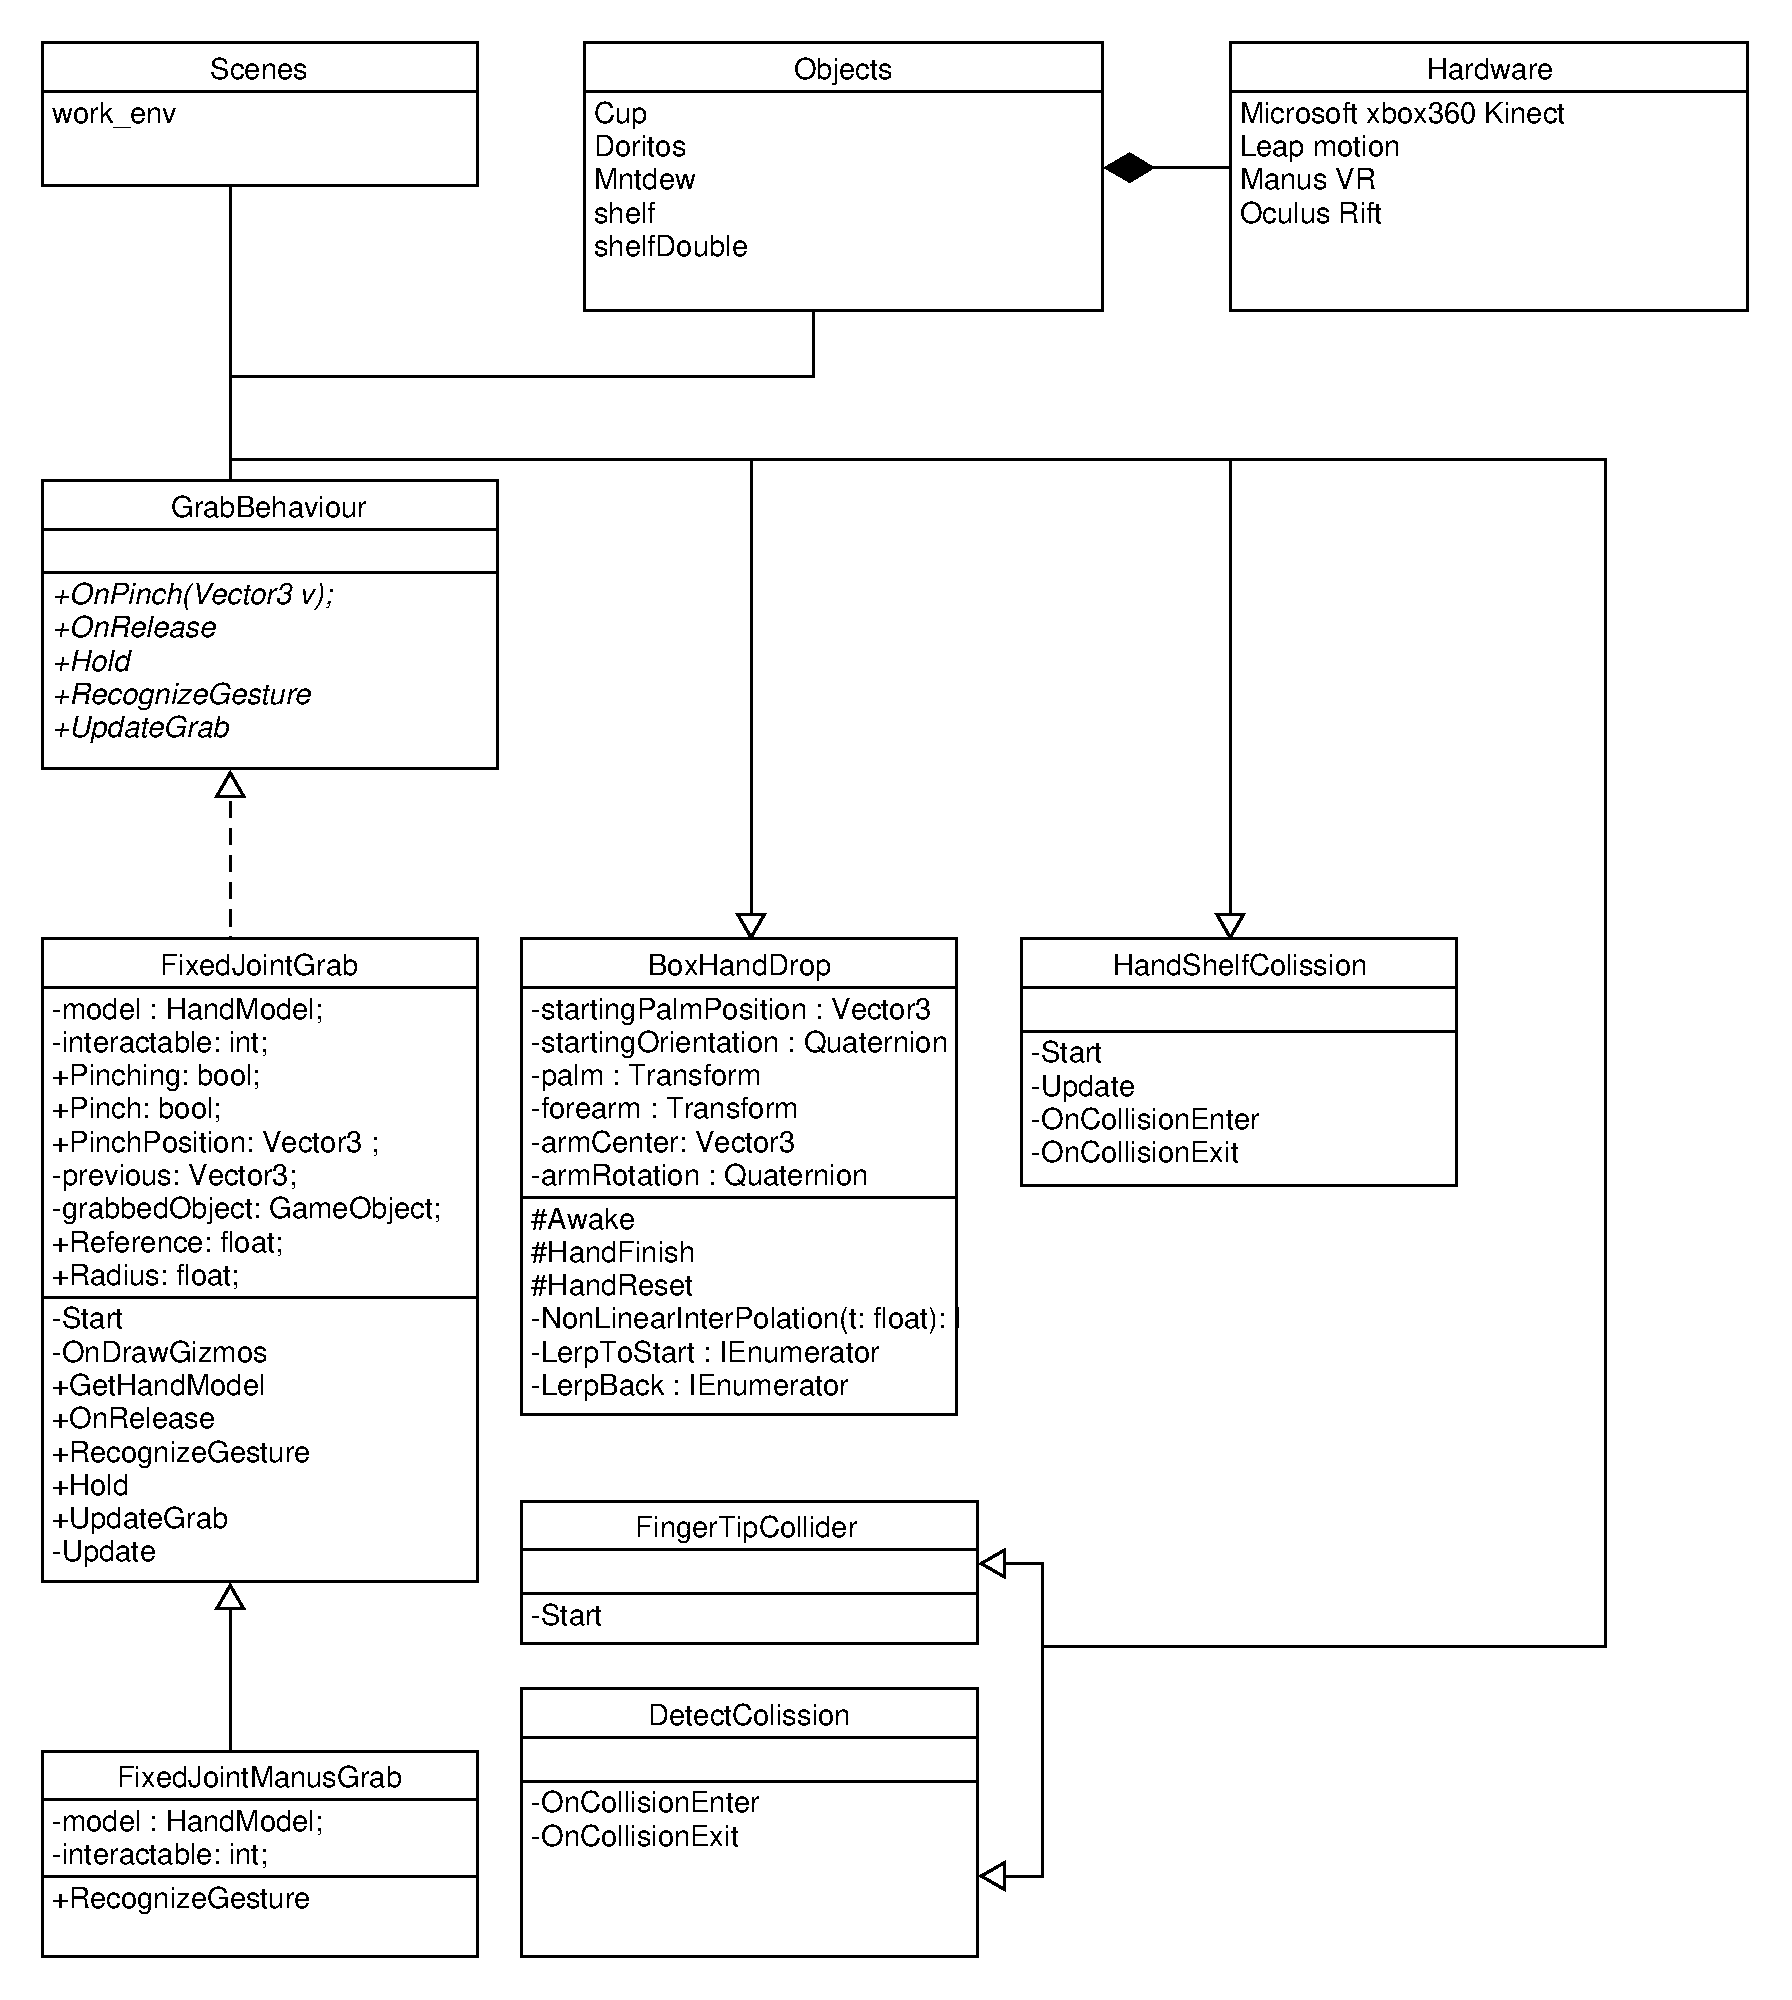
\includepdf[landscape=true, pages={1}]{CondExt_UML.pdf}

\end{document}
